\chapter{Testing}

\section{Website}

First the website is tested. The program on the second core is modified for the purpose of testing. Instead of correctly filtering the input its more important task will be periodically logging the value of alpha and beta to the serial line, even if it interferes with the timing of the DAC module.

\begin{figure}[H]
    \centering
    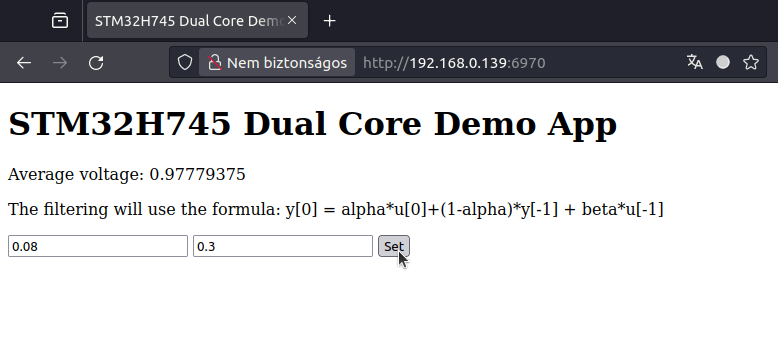
\includegraphics[width=150mm, keepaspectratio]{figures/webpage-test1.png}
    \caption{Webpage Before Inputting New Coefficients}
    \label{fig:webpage-test1}
\end{figure}

Inputting new values on the webpage to this modified program results in the following output on a terminal monitoring the serial port.

\begin{figure}[H]
    \centering
    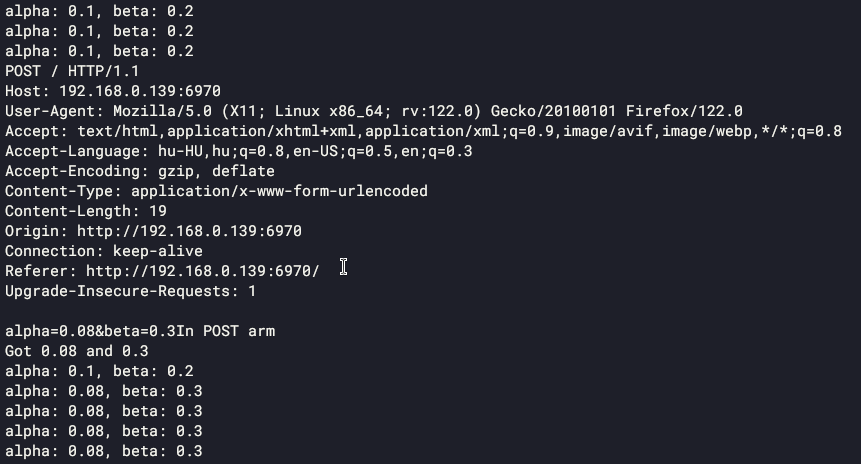
\includegraphics[width=150mm, keepaspectratio]{figures/coef-log.png}
    \caption{Serial Output when New Coefficients Are Supplied}
    \label{fig:coef-log}
\end{figure}

Supplying new variables refreshes the site, which is currently the only way to change the average voltage displayed. During the test a sine wave with an amplitude of 500 mv and offset of 1 V was supplied to the ADC.

\begin{figure}[H]
    \centering
    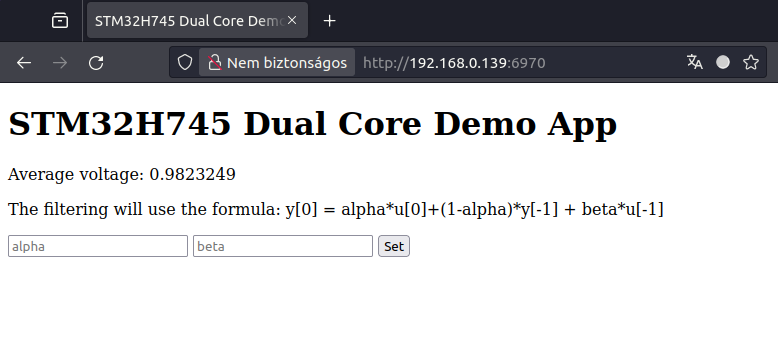
\includegraphics[width=150mm, keepaspectratio]{figures/webpage-test2.png}
    \caption{Webpage With Changed Average Voltage}
    \label{fig:webpage-test2}
\end{figure}

These results confirm that the two cores can communicate and exchange the necessary data. Also that the website works correctly is confirmed too.

\section{Low Pass Filter}

Testing the functionality of the second core required a tool that can generate an input and handle the output of the analog peripherals on the microcontroller. For this purpose a Picoscope 2000 series oscilloscope was used. It can act as a traditional digital oscilloscope and also generate arbitrary functions either based on common signals or a series of samples.

As a first step I tested the upper limit of the frequency the microcontroller can put out. In this configuration the M4 core was programmed to transform the 16 bit input from the ADC to a 12 bit output for the DAC, so essentially the input becomes the output without any modification. After some experimentation the limit came out at around 3 kHz, where the output is fairly well preserved.

\begin{figure}[H]
    \centering
    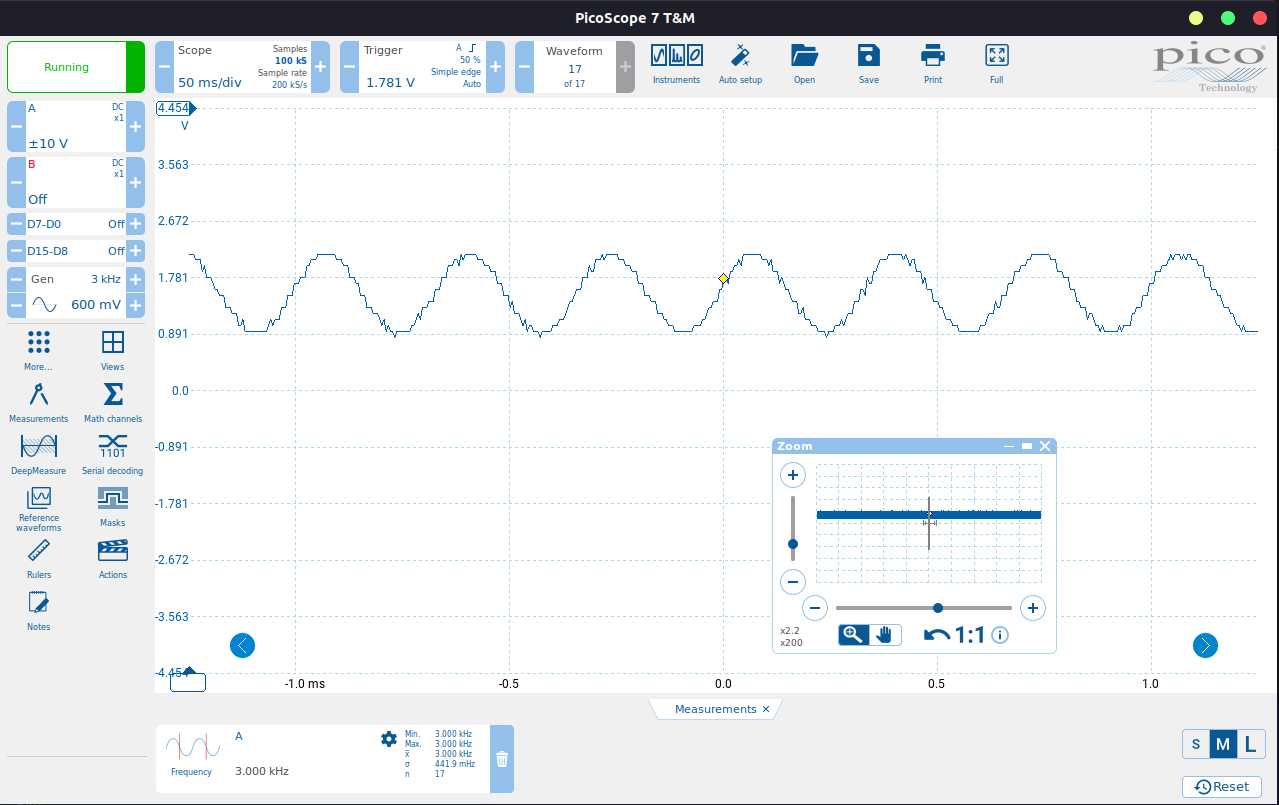
\includegraphics[width=150mm, keepaspectratio]{figures/upperlimit-good.png}
    \caption{Output of the DAC at 3 kHz}
    \label{fig:upperlimit-good}
\end{figure}

At around 8 kHz the signal lost its integrity. The shape of the sine wave is still visible but the amplitude is reduces, as there is not enough time for the DAC to settle properly.

\begin{figure}[H]
    \centering
    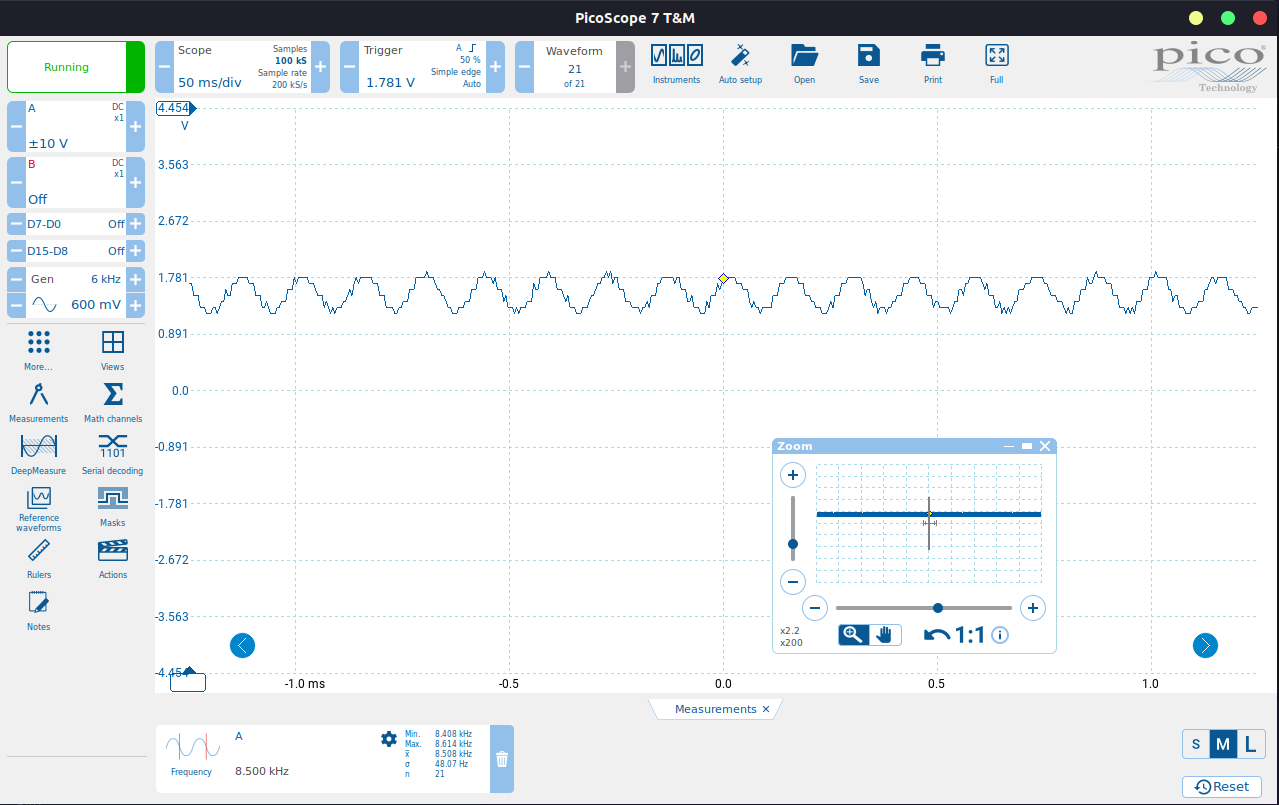
\includegraphics[width=150mm, keepaspectratio]{figures/upperlimit-bad.png}
    \caption{Output of the DAC at 8 kHz}
    \label{fig:upperlimit-bad}
\end{figure}

With this information, I started experimenting with the signal filtering. First I created an input, regular white noise added to a sine wave.

\begin{figure}[H]
    \centering
    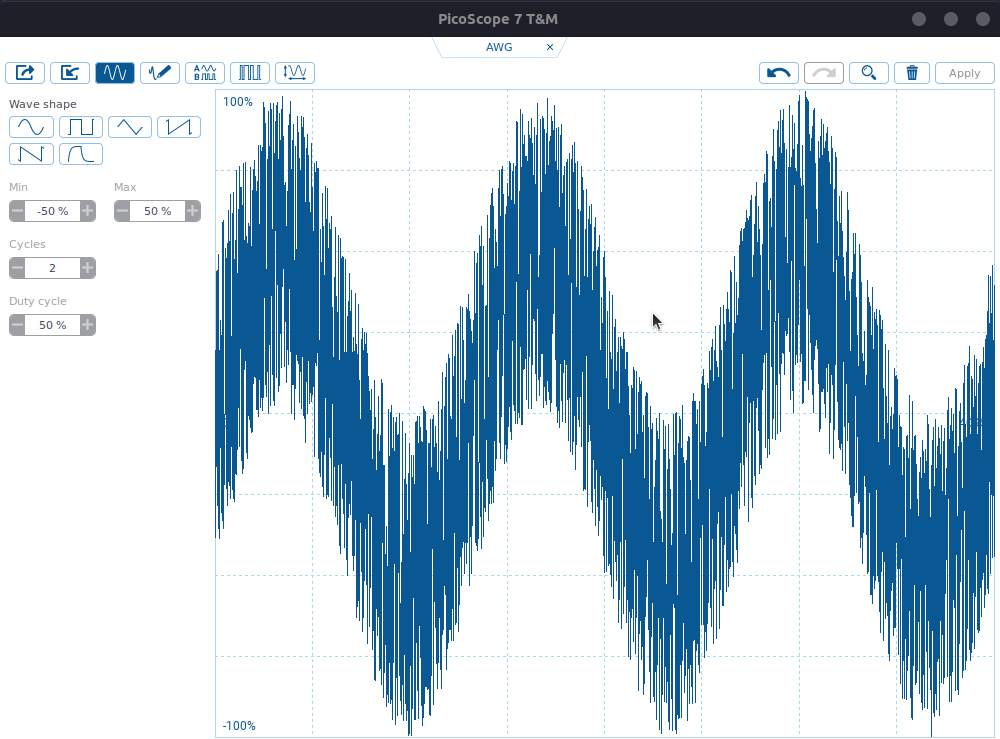
\includegraphics[width=150mm, keepaspectratio]{figures/sine-with-error.png}
    \caption{Samples of the Input Signal}
    \label{fig:sine-with-error}
\end{figure}

At first alpha is set to 1.0 and beta is set to 0.0, this configuration bypasses the filter entirely.

\begin{figure}[H]
    \centering
    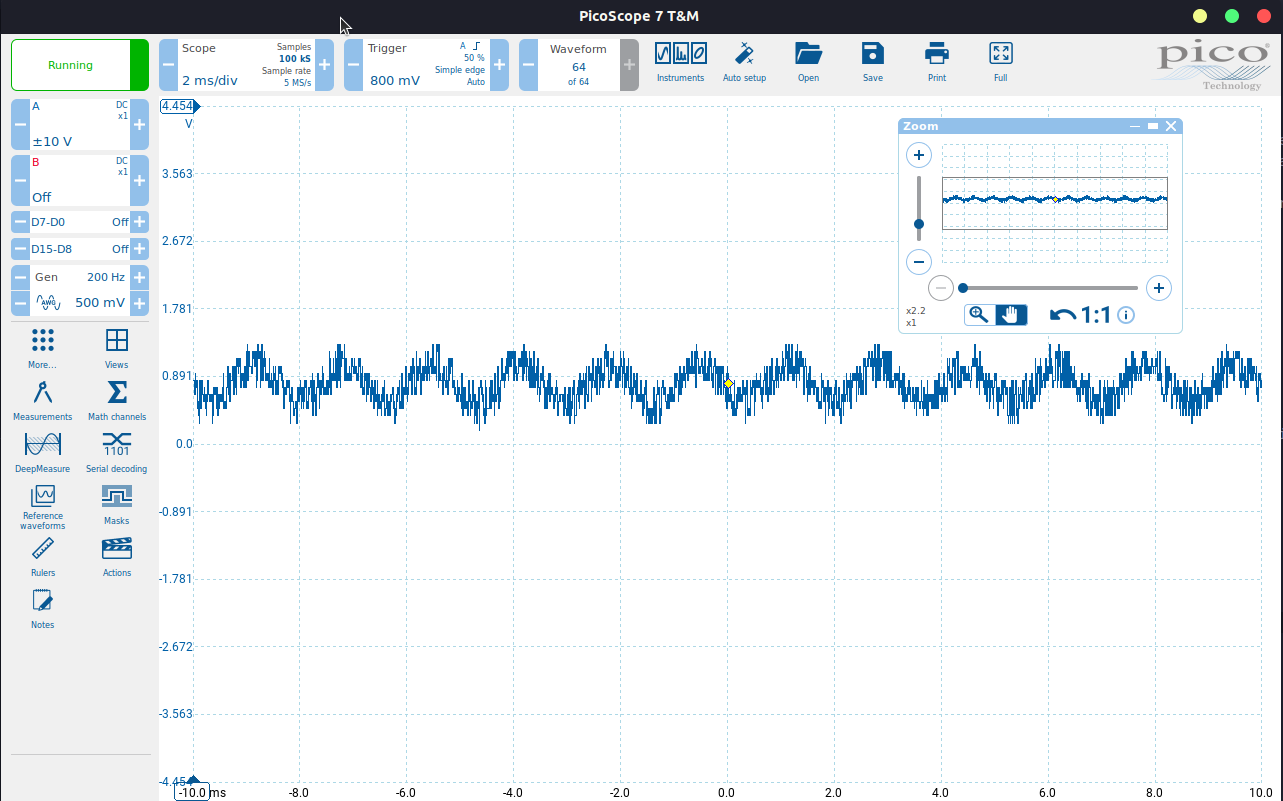
\includegraphics[width=150mm, keepaspectratio]{figures/bypass.png}
    \caption{Output without Filtering}
    \label{fig:bypass}
\end{figure}

The input has quite a bit of noise, so we will start experimenting with alpha at 0.2 while beta remains unchanged.

\begin{figure}[H]
    \centering
    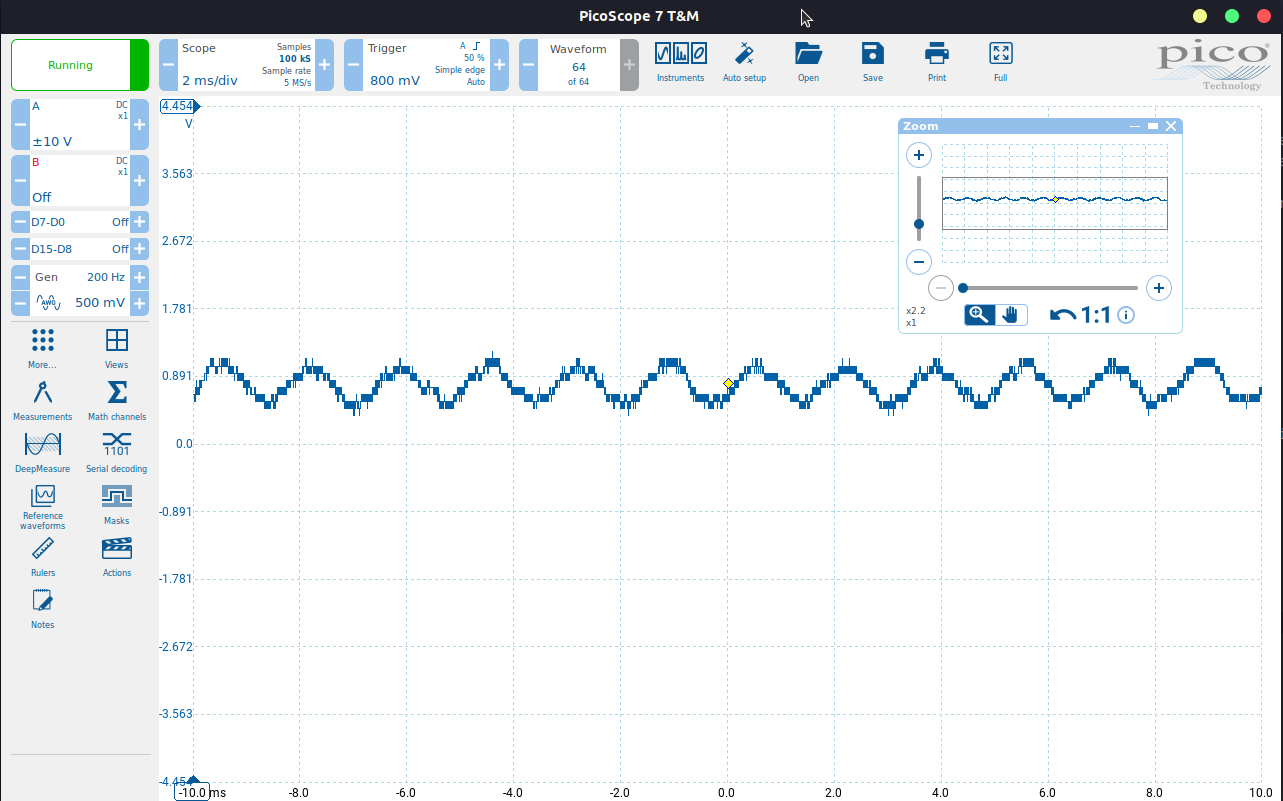
\includegraphics[width=150mm, keepaspectratio]{figures/alpha02.png}
    \caption{Output with alpha=0.2 and beta=0.0}
    \label{fig:alpha02}
\end{figure}

After some experimentation, selecting alpha=0.08 yields the most acceptable results.

\begin{figure}[H]
    \centering
    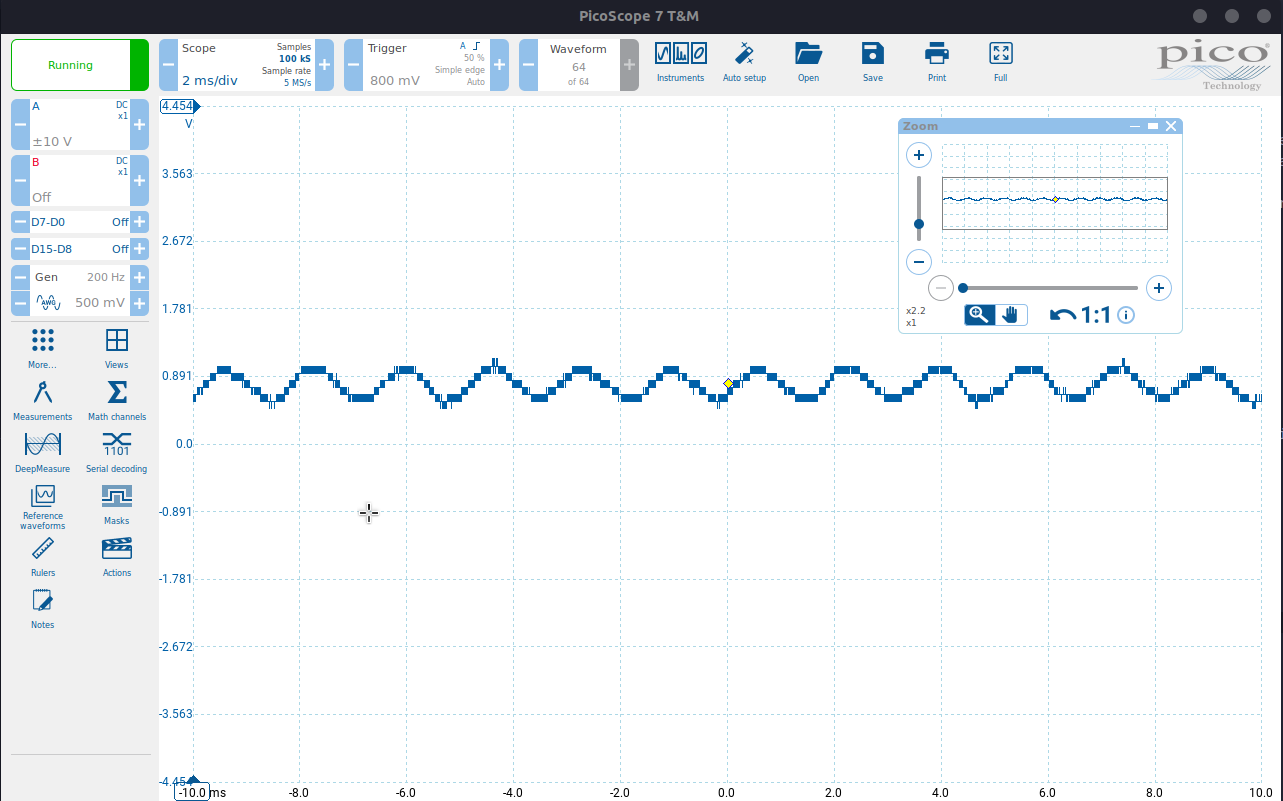
\includegraphics[width=150mm, keepaspectratio]{figures/alphaok.png}
    \caption{Output with alpha=0.08 and beta=0.0}
    \label{fig:alphaok}
\end{figure}

The beta coefficient causes the last input sample to be taken into account when calculating the output, which is useful in reducing infrequent spikes, but less so in reducing white noise.

\begin{figure}[H]
    \centering
    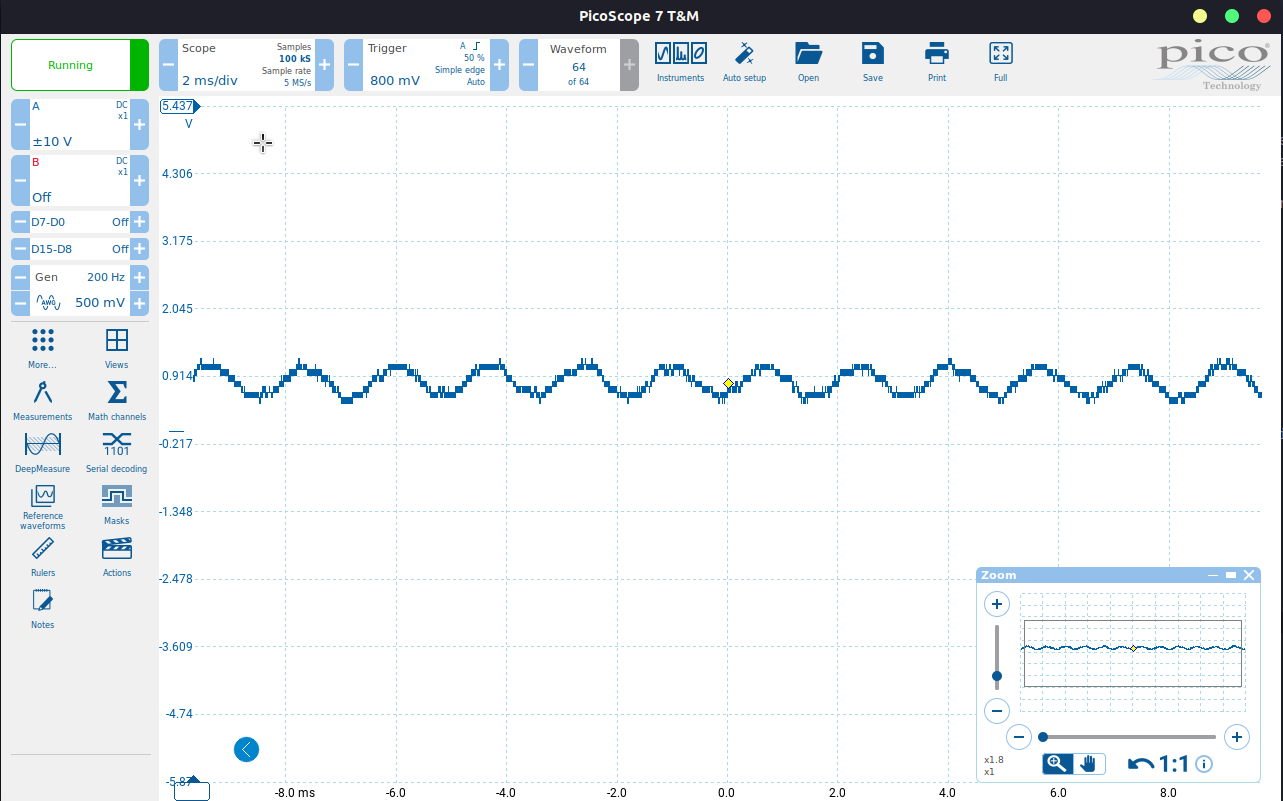
\includegraphics[width=150mm, keepaspectratio]{figures/beta.png}
    \caption{Output with alpha=0.2 and beta=0.2}
    \label{fig:beta}
\end{figure}

As expected, setting beta=0.2 did not influence the output at all.
